\section{Analyse}
	\subsection{Présentation des TAD}
		\subsubsection{TAD FichierTexte}
			\begin{tad}
	\tadNom{FichierTexte}
	%\tadParametres{Element,Clef}
	\tadDependances{\chaine, Mode, \caractere, \booleen}
	\begin{tadOperations}{ecrireCaractere}
		\tadOperation{fichierTexte}%
			{\tadUnParam{\chaine}}%
			{\tadUnParam{FichierTexte}}
		\tadOperationAvecPreconditions{ouvrir}%
			{\tadDeuxParams{FichierTexte}{Mode}}%
			{\tadUnParam{FichierTexte}}
		\tadOperationAvecPreconditions{fermer}%
			{\tadUnParam{FichierTexte}}%
			{\tadUnParam{FichierTexte}}
		\tadOperation{estOuvert}%
			{\tadUnParam{FichierTexte}}%
			{\tadUnParam{\booleen}}
		\tadOperationAvecPreconditions{Mode}%
			{\tadUnParam{FichierTexte}}%
			{\tadUnParam{Mode}}
		\tadOperationAvecPreconditions{finFichier}%
			{\tadUnParam{FichierTexte}}%
			{\tadUnParam{\booleen}}
		\tadOperationAvecPreconditions{ecrireChaine}%
			{\tadDeuxParams{FichierTexte}{\chaine}}%
			{\tadUnParam{FichierTexte}}
		\tadOperationAvecPreconditions{lireChaine}%
			{\tadUnParam{FichierTexte}}%
			{\tadDeuxParams{FichierTexte}{\chaine}}
		\tadOperationAvecPreconditions{ecrireCaractere}%
			{\tadDeuxParams{FichierTexte}{\caractere}}%
			{\tadUnParam{FichierTexte}}
		\tadOperationAvecPreconditions{lireCaractere}%
			{\tadUnParam{FichierTexte}}%
			{\tadDeuxParams{FichierTexte}{\caractere}}
	\end{tadOperations}
	\begin{tadSemantiques}{ecrireCaractere}
		\tadSemantique{FichierTexte}%
			{creation d’un fichier texte à partir d’un fichier identifié par son nom}
		\tadSemantique{ouvrir}%
			{ouvre un fichier texte en lecteur ou ecriture. Si le mode est ecriture et que le fichier existe, alors ce dernier est écrasé}
		\tadSemantique{fermer}%
			{ferme un fichier texte}
		\tadSemantique{lireCaractere}%
			{lit un caractère à partir de la position courante du fichier}
		\tadSemantique{lireChaine}%
			{lit une chaine (jusqu’à un retour à la ligne ou la fin de fichier) à partir de la position courante du fichier}
		\tadSemantique{ecrireCaractere}%
			{écrit un caractère à partir de la position courante du fichier}
		\tadSemantique{ecrireChaine}%
		{écrit une chaine suivie d’un retour à la ligne à partir de la position courante du fichier}
	\end{tadSemantiques}
	
	\begin{tadPreconditions}{ecrireCaractere}
		\tadPrecondition{ouvrir(f)}%
			{non estOuvert(f)}
		\tadPrecondition{fermer(f)}%
			{estOuvert(f)}
		\tadPrecondition{finFichier(f)}%
			{mode(f)=lecture}
		\tadPrecondition{lireXX}%
			{estOuvert(f) et mode(f)=lecture et non finFichier(f)}
		\tadPrecondition{ecrireXX}%
			{estOuvert(f) et mode(f)=ecriture}
	\end{tadPreconditions}
%	\begin{tadAxiomes}
%		\tadAxiome{dictionnaire()}
%	\end{tadAxiomes}
\end{tad}

			
		\subsubsection{TAD Mot}
			\begin{tad}
	\tadNom{Mot}
	\tadDependances{\chaine, \naturelNonNul, \caractere, \booleen}
	\begin{tadOperations}{Mot}
		\tadOperation{estUneLettre}%
			{\tadUnParam{\caractere}}%
			{\tadUnParam{\booleen}}
		\tadOperation{estUnMot}%
			{\tadUnParam{\chaine}}%
			{\tadUnParam{\booleen}}
		\tadOperationAvecPreconditions{creerMot}%
			{\tadUnParam{\chaine}}%
			{\tadUnParam{Mot}}
		\tadOperation{estAvantOrdreAlphabetique}%
			{\tadDeuxParams{Mot}{Mot}}%
			{\tadUnParam{\booleen}}
		\tadOperation{sontEgaux}%
			{\tadDeuxParams{Mot}{Mot}}%
			{\tadUnParam{\booleen}}
		\tadOperation{longueur}%
			{\tadUnParam{Mot}}%
			{\tadUnParam{NaturelNonNul}}
		\tadOperation{motEnChaine}%
			{\tadUnParam{Mot}}%
			{\tadUnParam{\chaine}}
		\tadOperationAvecPreconditions{remplacerLettre}%
			{\tadTroisParams{NaturelNonNul}{\caractere}{Mot}}%
			{\tadUnParam{Mot}}
		\tadOperationAvecPreconditions{supprimerLettre}%
			{\tadDeuxParams{NaturelNonNul}{Mot}}%
			{\tadUnParam{Mot}}
		\tadOperationAvecPreconditions{insererLettre}%
			{\tadTroisParams{\caractere}{Mot}{NaturelNonNul}}%
			{\tadUnParam{Mot}}
		\tadOperationAvecPreconditions{inverserLettre}%
			{\tadDeuxParams{NaturelNonNul}{Mot}}%
			{\tadUnParam{Mot}}
		\tadOperationAvecPreconditions{decomposerMot}%
			{\tadDeuxParams{Mot}{NaturelNonNul}}%
			{\tadDeuxParams{Mot}{Mot}}
	\end{tadOperations}
	
	\begin{tadSemantiques}{Mot}
		\tadSemantique{estUneLettre}%
			{renvoie vrai si l'\'el\'ement pris en entr\'e est une lettre (minuscule ou majuscule)}
		\tadSemantique{estUnMot}%
			{renvoie vrai si la chaîne de caract\`eres est non vide et que tous ses caract\`eres sont des lettres.}
		\tadSemantique{creerUnMot}%
			{cr\'e\'e un mot \`a partir d’une cha\^ine de caract\`eres.}
		\tadSemantique{estAvantOrdreAlphabetique}%
			{retourne vrai si le premier mot mis en param\`etre est avant le second dans l'ordre alphab\`etique.)}
		\tadSemantique{sontEgaux}%
			{retourne vrai si les mots sont identiques (non sensible à la casse)}
		\tadSemantique{longueur}%
			{calcule la longueur d'un mot}
		\tadSemantique{motEnChaine}%
			{transforme un mot en cha\^ine de caract\`eres}
		\tadSemantique{remplacerLettre}%
			{remplace une lettre \`a un certain indice du mot}
		\tadSemantique{supprimerLettre}%
			{supprime une lettre \`a un certain indice du mot}
		\tadSemantique{insererLettre}%
			{ins\`ere une lettre \`a un certain indice du mot}
		\tadSemantique{inverserLettre}%
			{inverse deux lettres cons\'ecutives du mot}
		\tadSemantique{decomposerMot}%
			{décompose un mot en deux mots}
	\end{tadSemantiques}
	
	\begin{tadPreconditions}{Mot}
		\tadPrecondition{creerMot(c)}%
			{estUnMot(c)}
		\tadPrecondition{remplacerLettre(i, car, mot)}%
			{i$\leq$longueur(mot)}
		\tadPrecondition{supprimerLettre(i, mot)}%
			{i$\leq$longueur(mot)}
		\tadPrecondition{insererLettre(c, mot, i)}%
			{i$\leq$longueur(mot) + 1}
		\tadPrecondition{inverserLettre(i, mot)}%
			{i < longueur(mot)}
		\tadPrecondition{decomposerMot(mot, i)}%
			{1 < i < longueur(mot)}
	\end{tadPreconditions}
	
\end{tad}

			
		\subsubsection{TAD Dictionnaire}
			\begin{tad}
	\tadNom{Dictionnaire}
	\tadParametres{}
	\tadDependances{fichierTexte, Dictionnaire, Mot, \booleen, mode, \entier}
	\begin{tadOperations}{Dictionnaire}
		\tadOperation{dictionnaire}%
			{}%
			{\tadUnParam{Dictionnaire}}
		\tadOperation{estVide}%
			{\tadUnParam{Dictionnaire}}%
			{\tadUnParam{\booleen}}
		\tadOperation{estPresent}%
			{\tadDeuxParams{Dictionnaire}{Mot}}%
			{\tadUnParam{\booleen}}
		\tadOperation{hauteur}%
			{\tadUnParam{Dictionnaire}}%
			{\tadUnParam{\entier}}	
		\tadOperationAvecPreconditions{faireSimpleRotationDroite}%
			{\tadUnParam{Dictionnaire}}%
			{\tadUnParam{Dictionnaire}}	
		\tadOperationAvecPreconditions{faireSimpleRotationGauche}%
			{\tadUnParam{Dictionnaire}}%
			{\tadUnParam{Dictionnaire}}	
		\tadOperationAvecPreconditions{faireDoubleRotationDroite}%
			{\tadUnParam{Dictionnaire}}%
			{\tadUnParam{Dictionnaire}}
		\tadOperationAvecPreconditions{faireDoubleRotationGauche}%
			{\tadUnParam{Dictionnaire}}%
			{\tadUnParam{Dictionnaire}}
		\tadOperationAvecPreconditions{reequilibrer}%
			{\tadUnParam{Dictionnaire}}%
			{\tadUnParam{Dictionnaire}}		
		\tadOperationAvecPreconditions{ajouterMot}%
			{\tadDeuxParams{Dictionnaire}{Mot}}%
			{\tadUnParam{Dictionnaire}}
		\tadOperationAvecPreconditions{ajouterFichier}%
			{\tadDeuxParams{Dictionnaire}{\chaine}}%
			{\tadUnParam{Dictionnaire}}
		\tadOperationAvecPreconditions{chargerDictionnaire}%
			{\tadUnParam{\chaine}}%
			{\tadUnParam{Dictionnaire}}
		\tadOperationAvecPreconditions{enregistrerDictionnaire}%
			{\tadDeuxParams{Dictionnaire}{\chaine}}%
			{\tadUnParam{}}
		
	\end{tadOperations}
	
	\begin{tadSemantiques}{Dictionnaire}
		\tadSemantique{dictionnaire}%
			{cr\'e\'e un dictionnaire vide.}
		\tadSemantique{estVide}%
			{retourne VRAI si le dictionnaire est vide.}
		\tadSemantique{estPresent}%
			{retourne VRAI si le mot est pr\'esent dans le dictionnaire.}
		\tadSemantique{hauteur}%
			{retourne la hauteur du dictionnaire.}
		\tadSemantique{faireSimpleRotationDroite}%
			{retourne le dictionnaire après lui avoir appliqué une simple rotation à droite.}
		\tadSemantique{faireSimpleRotationGauche}%
			{retourne le dictionnaire après lui avoir appliqué une simple rotation à gauche.}
		\tadSemantique{faireDoubleRotationDroite}%
			{retourne le dictionnaire après lui avoir appliqué une double rotation à droite.}
		\tadSemantique{faireDoubleRotationGauche}%
			{retourne le dictionnaire après lui avoir appliqué une double rotation à gauche.}
		\tadSemantique{reequilibrer}%
			{retourne le dictionnaire après avoir rééquilibré ses branches.}
		\tadSemantique{ajouterMot}%
			{ajoute un mot dans le dictionnaire.}
		\tadSemantique{ajouterFichier}%
			{ajoute les mots d’un fichier texte dans le dictionnaire.}
		\tadSemantique{chargerDictionnaire}%
			{charge un dictionnaire \`a partir d’un fichier texte.}
		\tadSemantique{enregistrerDictionnaire}%
			{cr\'e\'e un fichier texte contenant le dictionnaire mis en paramètre.}
	\end{tadSemantiques}
	
	\begin{tadPreconditions}{Dictionnaire}
		\tadPrecondition{faireSimpleRotationDroite(dictionnaire)}%
			{non(estVide(dictionnaire)) ET non(estVide(obtenirFilsGauche(dictionnaire)))}
		\tadPrecondition{faireSimpleRotationGauche(dictionnaire)}%
			{non(estVide(dictionnaire)) ET non(estVide(obtenirFilsDroit(dictionnaire)))}
		\tadPrecondition{faireDoubleRotationDroite(dictionnaire)}%
			{non(estVide(dictionnaire) ET non(estVide(obtenirFilsGauche(dictionnaire))) ET
non(estVide(obtenirFilsDroit(obtenirFilsGauche(dictionnaire))))}
		\tadPrecondition{faireDoubleRotationGauche(dictionnaire)}%
			{non(estVide(dictionnaire)) ET non(estVide(obtenirFilsDroit(dictionnaire)) ET non(estVide(obtenirFilsGauche(obtenirFilsDroit(dictionnaire))))}
		\tadPrecondition{reequilibrer(dictionnaire)}%
			{non(estVide(dictionnaire)) ET abs(hauteur(obtenirFilsGauche(dictionnaire)) - hauteur(obtenirFilsDroit(dictionnaire))) = 2}
		\tadPrecondition{ajouterMot(dictionnaire, mot)}%
			{non(estPresent(m))}
		\tadPrecondition{ajouterFichier(dictionnaire, nomFichier)}%
			{nomFichier != ""}
		\tadPrecondition{chargerDictionnaire(nomFichier)}%
			{nomFichier != ""}
		\tadPrecondition{enregistrerDictionnaire(dictionnaire, nomFichier)}%
			{nomFichier != ""}
	\end{tadPreconditions}
	
	%\begin{tadAxiomes}
		%\tadAxiome{dictionnaire()}
	%\end{tadAxiomes}
\end{tad}

			
		\subsubsection{TAD CorrecteurOrthographique}
		Dans le TAD ci-dessous ne sont pas mentionnées les fonctions et procédures basiques permettant de manipuler les tableaux. En effet, seules celles constituant l'architecture principale de notre correcteur orthographique sont ajoutées ici. 
			\begin{tad}
	\tadNom{CorrecteurOrthographique}
	%\tadParametres{}
	\tadDependances{Mot, Dictionnaire, \booleen, NaturelNonNul }
	\begin{tadOperations}{CorrecteurOrthographique}
		\tadOperation{chainesEnMots}%
			{\tadUnParam{\chaine}}%
			{\tadDeuxParams{Liste <Mot>}{Liste <Naturel>}}
		\tadOperation{sontPresents}%
			{\tadDeuxParams{Liste <Mot>}{Dictionnaire}}%
			{\tadUnParam{Liste <\booleen>}}
		\tadOperation{proposerMots}%
			{\tadDeuxParams{Mot}{Dictionnaire}}%
			{\tadUnParam{Ensemble <Mot>}}
		\tadOperation{proposerMotsListe}%
			{\tadDeuxParams{Liste <Mot>}{Dictionnaire}}%
			{\tadDeuxParams{Liste <Ensemble <Mot>>}{Liste <\booleen>}}
	\end{tadOperations}
		
	\begin{tadSemantiques}{CorrecteurOrthographique}
		\tadSemantique{chainesEnMots}%
			{transforme une cha\^ine de caract\`eres en une liste de Mot et renvoie aussi une liste de la position de chaque mot}
		\tadSemantique{sontPresents}%
			{renvoie une liste de Booleen indiquant la présence ou non des mots de la liste}
		\tadSemantique{proposerMots}%
			{donne un ensemble de Mot correspondant aux corrections possibles d’un mot mal orthographi\'e}
		\tadSemantique{proposerMotsListe}%
			{envoie la liste des ensembles de Mot corrig\'es possible pour les mots qui ne sont pas dans le dictionnaire}
	\end{tadSemantiques}
		
		%\begin{tadAxiomes}
			%\tadAxiome{CorrecteurOrthographique}
		%\end{tadAxiomes}
		
\end{tad}

			
		\subsection{Analyse Descendante}
			\begin{center}
			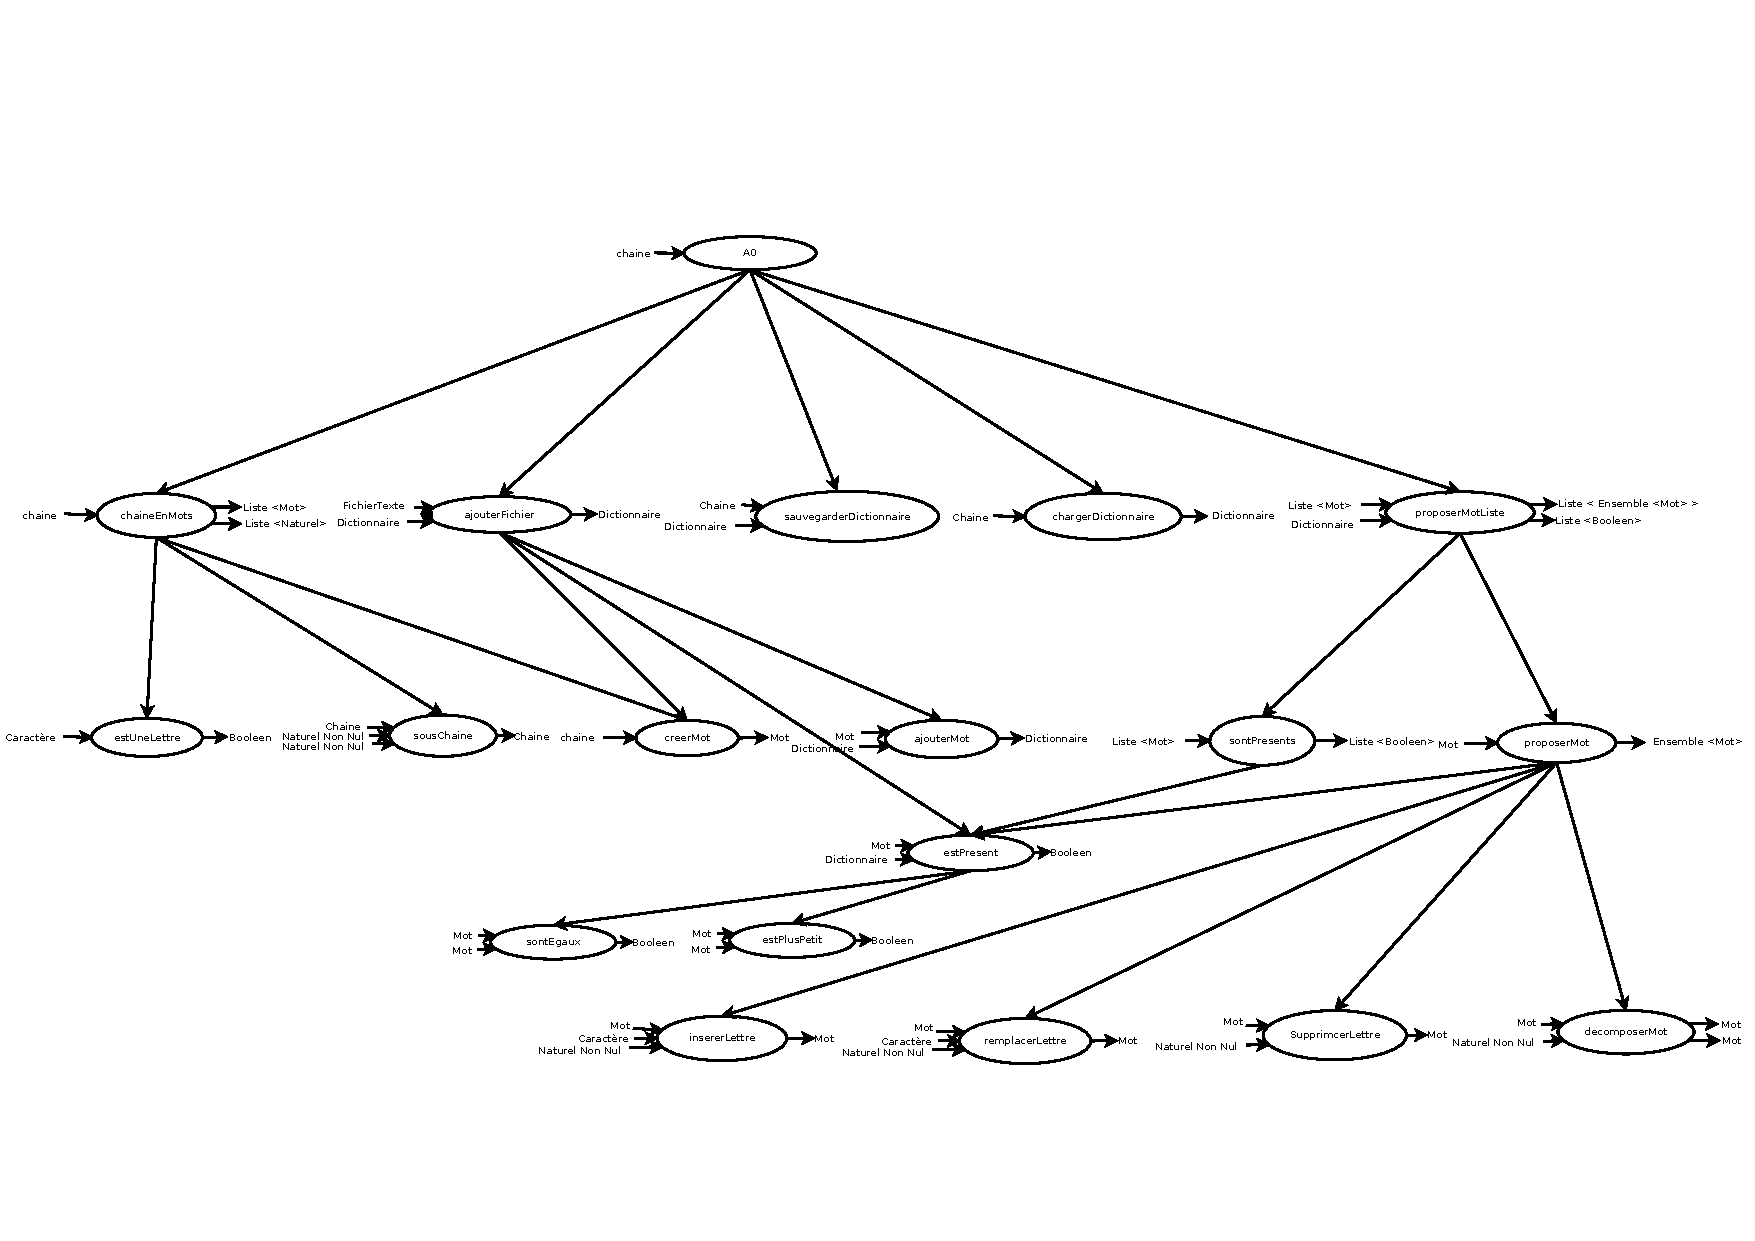
\includegraphics[scale=0.6]{images/AnalyseDescendante.pdf}
			\end{center}
